\documentclass[10pt,letterpaper]{article}
%%%%%%%%% PACKAGES %%%%%%%%%%

\usepackage[T1]{fontenc}        %finden von umlaugen ermöglichenver
\usepackage{acronym}

\usepackage{longtable}
\usepackage{listings}
\usepackage{titlesec}
\titleformat{\paragraph}[hang]{\normalfont\bfseries}{}{0pt}{}
\usepackage{url}

\usepackage{pslatex} 
\usepackage{graphicx} % Standardgrafikpacket
\usepackage[american]{babel}
\usepackage{fixltx2e} % Fixes for LaTeX
\usepackage{ragged2e}
\usepackage[sort,numbers,super]{natbib}
\usepackage{upgreek}

\marginparwidth2.5cm 
\marginparsep0.5cm
\setlength{\parskip}{1ex}
\usepackage[automark]{scrpage2}
\usepackage[usenames,dvipsnames]{color}

% Schönheiten %%%%%%%%%%%%%%%%%%%%%%%%%%%%%%%%%%%%%%%%%%%%%%%%%%%%%%%%%%%%%
\usepackage{setspace} % Set space between lines
%\usepackage[linkcolor=black,dvips=true,citecolor=black,linkcolor=black,colorlinks=true]{hyperref} % schöne schwarze Links
\usepackage[format=plain,margin=5pt,font=small,textfont=footnotesize,labelsep=endash,labelfont=bf]{caption} % verschönerung der captions etc
\usepackage{subcaption}


% Texterweiterungen %%%%%%%%%%%%%%%%%%%%%%%%%%%%%%%%%%%%%%%%%%%%%%%%%%%%%%%
\usepackage{amsmath} % Additional math
\usepackage{amssymb}
\usepackage{textcomp} % Text companion extended symbols


\begin{document}



\begin{flushleft}
{\Large
\textbf\newline{Using embedding spaces to visualize and guide refinement of a simple CNN}
}
\newline
% authors go here:
\\
Peter Rupprecht\textsuperscript{1,2},
Stephan Gerhard\textsuperscript{1},
Rainer Friedrich\textsuperscript{1,2}
\\
\bigskip
1 Friedrich Miescher Institute for Biomedical Research, Maulbeerstrasse 66, CH-4058 Basel, Switzerland
\\
2 University of Basel, Basel 4003, Switzerland
\\

\end{flushleft}

\subsection*{Basic CNN structure}

In order to infer a spike probability for time bin $j$ (Fig. \ref{fig_rupp1}A), we used the calcium trace located around $j$, including 25\% before and 75\% after $j$, totaling to 128 samples, \textit{i.e.}, 1.28 sec (Fig. \ref{fig_rupp1}C). We trained a convolutional neural network to use these 128-wide windows to predict the corresponding spiking probability. To facilitate gradient ascent, we smoothed the discrete spiking ground truth with a Gaussian filter ($\sigma = \sqrt 2$ sec, Fig. \ref{fig_rupp1}B).

We implemented the convolutional neural network in Python using Keras\cite{chollet2015keras} with the Tensorflow\cite{tensorflow2015-whitepaper} backend. The network architecture is shown in Fig. \ref{fig_rupp1}. The convolutional filter size, particularly for the first layer, was chosen rather large, since simple CNNs with 3 or 4 convolutional layers with small input filter sizes (3, 5 or 7) performed poorly (data not shown). No zero-padding was used. The numbers of filters were chosen to increase with depth in order to allow for a larger capacity to represent higher-order features. Standard \textit{relu} activation units were used after each convolutional and dense layer, except for the last dense layer, where a linear activation was used to allow the output of continuous spiking probabilities.

All parameters were chosen based on intuition gained through a small exploratory hyperparameter study using diverse 3- and 4-layer CNNs with varying filter sizes, filter numbers and input window sizes. We tried to control overfitting by randomly omitting single neurons from the training data and checking predictive performance of the CNN model for the respective omitted neuron.

\subsection*{Generation of an embedding space based on mutual predictive power}

Although the above-described CNN performed well when it came to fitting single datasets of the ground truth, one single model trained on all datasets usually performed not as well for any of the datasets as the same CNN trained on the respective dataset alone. To better understand this, we wanted to quantify how well a model that had been fitted to predict spikes for neuron $i$ can make the same kind of predictions for neuron $j$. To this end, we fitted a low-capacity CNN (with two locally connected convolutional layers and one dense layer) for each neuron $i$. The small size of the network together with a high dropout rate during training (50\% after each layer) was used to prevent overfitting. This model was then applied to predict spiking probabilities both for neuron $i$ and all neurons $j \neq i$. This matrix of 'predictive power' (measured with the Pearson correlation coefficient between prediction and ground truth, identical to the evaluation of the Spikefinder competition), is shown in Fig. \ref{fig_rupp2}A. For instance, row 55 shows how well spikes of neuron 55 can be predicted by the networks generated by all other neurons. Column 55, on the other hand, shows how well the model generated by neuron 55 can predict spikes of other neurons. The 5\% neurons that were worst at predicting their own spiking were discarded from the following modeling, assuming bad recording quality that is not suited for inclusion into a training dataset.

Normalization over columns, symmetrization of the matrix and averaging over datasets yields a matrix of predictive power, generating a matrix of proximity in prediction-space between datasets (Fig. \ref{fig_rupp2}B). A PCA of this matrix results in an embedding space that we limited to two dimensions due to the low number of datasets. Datasets close to each other in the embedding space (e.g. 2 and 4) can predict each other's spikes very well, whereas datasets distant from each other in space (e.g. datasets 4 and 5) fail to do so.

\begin{figure}[bt]
\centering
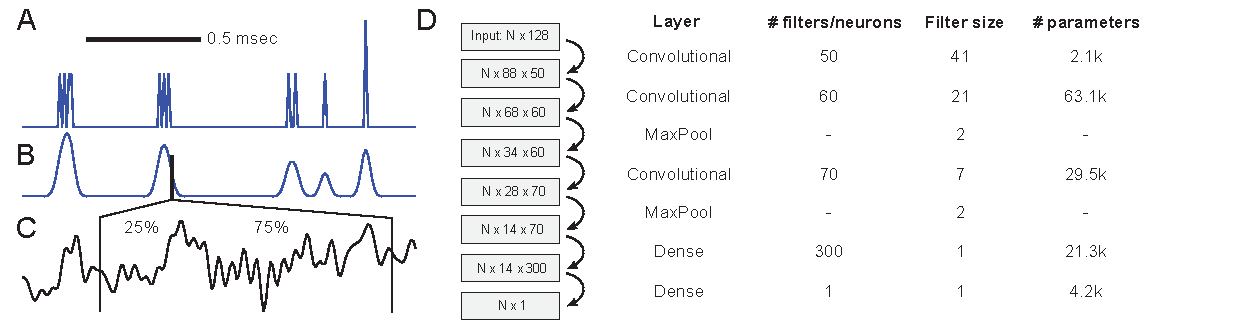
\includegraphics[width=0.95\textwidth]{images/ConvolutionalNet}
\caption{The basic convolutional neural network. \textbf{A,B}. The spiking ground truth was smoothed to facilitate gradient descent. \textbf{C}. For each time point of the smoothed spiking trace, a 1.28~sec time window of the calcium trace was selected. \textbf{D}. The $N$ inputs were transformed using a neural network with three convolutional layers. The numbers in the boxes indicate the output size of the respective layers.}
\label{fig_rupp1}
\end{figure}

\subsection*{Generation of an embedding space based on the similarity of statistical properties}

Using this approach, it is however not yet possible to map a neuron of a new dataset of unknown properties onto the right location of the embedding space above. To solve this problem, we calculated the following statistical properties of the raw calcium time traces (Fig. \ref{fig_rupp2}D):
\begin{itemize}
\item coefficient of variation, kurtosis, skewness
\item autocorrelation of the calcium time trace with its future value in 0.5, 1 and 2 seconds
\item generalized Hurst exponents of order 1-5
\item the power spectral density at different frequencies between 0.1 and 3.6 Hz
\end{itemize}
We did not attempt to find a minimal set of predictive properties to reduce computation time here, but used dimensional reduction techniques to automatically extract the relevant independent components. After averaging the standardized values over datasets (Fig. \ref{fig_rupp2}E), we used the two first principal components to generate a map of proximity in statistical property space (Fig. \ref{fig_rupp2}F). This map was generated using the training datasets (numbers located on the right side of the symbols). Test datasets were mapped into this PCA space (numbers on the left side of the symbols).

To generate a mapping between the locations of the datasets in the two embedding spaces, we fitted a simple regressor (\textit{DecisionTreeRegressor} from the scikit-learn package \cite{scikit-learn}) to the training datasets (schematic arrows in Fig. \ref{fig_rupp2}C,F). We then used this mapping to determine the position of the test datasets in the embedding space of mutual predictive power.

\begin{figure}[tb]
\centering
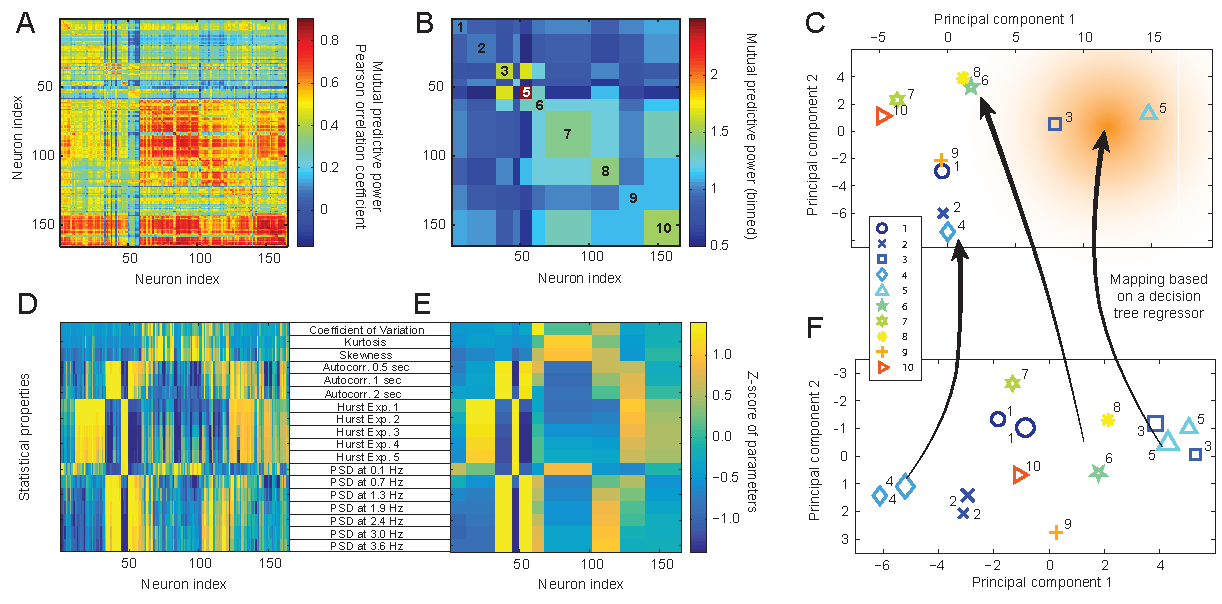
\includegraphics[width=0.95\textwidth]{images/EmbeddingSpaces}
\caption{Using embedding spaces to choose datasets for focused retraining. \textbf{A.} Matrix of mutual predictive power, measured using the Pearson correlation coefficient between prediction and ground truth. \textbf{B.} Same as (A), but normalized for columns and binned to datasets. \textbf{C.} Principal component analysis applied to (B), keeping the first two PCs. \textbf{D.} Statistical parameters quantified for single neurons, standardized. \textbf{E.} Same as (D), but binned for datasets. \textbf{F.} 2D principal component space generated using (E). Symbols with numbers to the right are from training datasets, used to span the PCA space; symbols with numbers to the left are from the test dataset and were projected into the PCA space.}
\label{fig_rupp2}
\end{figure}

\subsection*{Retraining of the basic model within a local environment of the embedding space}

Once the position in the embedding space is known for a dataset, the model that had been trained before on all datasets is retrained, but preferentially with neurons from datasets that lie close to the position in the embedding space. We weighted this preference with a function that decays exponentially over distance in the embedding space, as indicated by the red shading in Fig. \ref{fig_rupp2}C. Again, the functional form of the decay and the decay constant have been chosen heuristically without systematic optimization, since our goal was to showcase the power of our embedding space approach rather than finding a global optimum.

\subsection*{Embedding spaces as an intuitive interface to understand model selection}

This focused re-training is reminiscent of other approaches to conditional computation based on attention mechanisms. Given that any attention-based network can be replaced by a large enough not explicitly conditional network,\cite{bengio2013estimating} it seems clear that a large-enough CNN could make the embedding spaces dispensable without compromising performance, provided that regularization is properly performed. For example, a deep network could be used to learn the mapping from the raw time traces to the position in the predictive embedding space in Fig. \ref{fig_rupp2}C, replacing our explicit mapping based on extracted statistical properties. A powerful enough network applied to the original task of mapping calcium traces to spikes would include this mapping implicitly in its internal structure.

However, embedding spaces as a visual and explicit intermediate step for model refinement are more easily accessible for users, allow the use of relatively small convolutional neuronal networks and can highlight similarities and differences between datasets. For example, it is interesting to see that in both embedding spaces, datasets 3 and 5 cluster together, whereas dataset 8, which uses the same calcium indicator (GCaMP6s) in the same brain region (V1), is in proximity of dataset 6 (GCaMP5k in V1). Similarly, the datasets that use OGB-1 as indicator (1,2 and 4) tend to occupy similar regions of the embedding spaces, but datasets 1 and 2 which have both indicator and brain region (V1) in common, do not cluster in an obvious manner.

This indicates that model selection is not only based on the calcium indicator and the brain region, but on hidden parameters, \textit{e.g.}, signal-to-noise of the calcium recording, sampling rate, spike rate, temperature, indicator concentration, or others. To reliably comprise these possible hidden parameters with embedding spaces, it will be necessary to increase the number of datasets in order to support as many possible types of datasets as possible. However, the unknown dimensionality of this hidden parameter space makes it difficult to predict how many datasets would be required.

All of the code together with instructions on a) how to use it to reproduce our results and b) how to apply the networks on unknown calcium imaging data for deconvolution can be found online on Github \cite{ruppprecht2017embeddingspace}. 

%Train:
%    0.5410    0.4800    0.4920    0.5950    0.5320
%    0.5170    0.4950    0.4810    0.5630    0.3980
%Test
%    0.5950    0.4140    0.4340    0.3650    0.4960
%    0.5977    0.4230    0.3980    0.3720    0.4230

\footnotesize{
\RaggedRight	
\bibliography{elephant}
\bibliographystyle{apalike}
}

\end{document}

